Overall, the RNGs that we implemented performed as expected. All RNGs (with the notable and expected exception of RANDU) passed the majority of the tests, with at most one failure, and a few weak results which could very possibly pass if tested with different seeds. Statistics for passes, weaks, and failures are presented in visual form in Figure~\ref{fig:passesweaksfails} and tabularly in Table~\ref{tab:passesweaksfails}.

\begin{figure}[tb]
    \begin{center}
        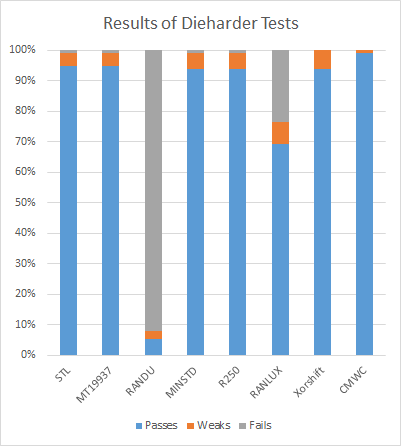
\includegraphics[width=\linewidth]{figures/passesweaksfails.png}
    \end{center}
    \caption{Percentage bar graph of results of Dieharder test results for implemented RNGS.}
    \label{fig:passesweaksfails}
\end{figure}

% http://www.tablesgenerator.com/
\begin{table}[tb]
    \caption{Table displaying Dieharder results for the implemented RNGs.}
    \label{tab:speed}
    \begin{center}
        \begin{tabular}{l|ccc}
        \hline
        \hline
\textbf{RNG Name} & \textbf{Passes} & \textbf{Weaks} & \textbf{Fails} \\
        \hline
STL               & 108             & 5              & 1              \\
MT19937           & 108             & 5              & 1              \\
RANDU             & 6               & 3              & 105            \\
MINSTD            & 107             & 6              & 1              \\
R250              & 107             & 6              & 1              \\
RANLUX            & 79              & 8              & 27             \\
Xorshift          & 107             & 7              & 0              \\
CMWC              & 113             & 1              & 0 \\
        \hline
        \hline
        \end{tabular}
    \end{center}
\end{table}


Another metric worth measuring is RNG speed. This metric has been alluded, but is formally measured in random numbers per second. Luckily, Dieharder generates this metric already. As expected, the STL implementation of the Mersenne Twister is quite fast (as is much of the STL), and the RANLUX implementation is slow (because it must discard so many numbers to keep the quality of output high). Of the other RNGs, our Mersenne Twister is the most complicated, and as a result it is the slowest. RANDU is simple and fast, and the other algorithms hover around the same speed. The data is presented graphically in Figure~\ref{fig:speed} and tabularly in Table~\ref{tab:speed}

It is important to remember that these speeds must be considered to be relative. These RNGs must be piped through the shell, as opposed to the GNU Scientific Library RNGs built into the Dieharder binary, and as a result, they are a factor of <placeholder> faster.

\begin{figure}[tb]
    \begin{center}
        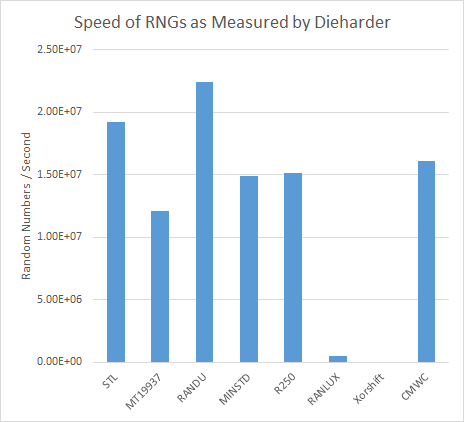
\includegraphics[width=\linewidth]{figures/speed.png}
    \end{center}
    \caption{Speed of implemented RNGs in random numbers per second as measured by Dieharder.}
    \label{fig:speed}
\end{figure}

% http://www.tablesgenerator.com/
\begin{table}[tb]
    \caption{Table displaying speeds of implemented RNGs as measured by Dieharder.}
    \label{tab:passesweaksfails}
    \begin{center}
        \begin{tabular}{l|c}
        \hline
        \hline
\textbf{RNG Name} & \textbf{Speed} \\
        \hline
STL       &  1.91E+07  \\
MT19937   &  1.26E+07  \\
RANDU     &  2.18E+07  \\
MINSTD    &  1.49E+07  \\
R250      &  1.51E+07  \\
RANLUX    &  5.00E+05  \\
Xorshift  &  7.90E+06  \\
CMWC      &  4.30E+06  \\
TinyMT    &  7.97E+06  \\

        \hline
        \hline
        \end{tabular}
    \end{center}
\end{table}

